%!TEX root = main.tex





\subsection{Successive Halving for Infinite-armed Bandits}\label{theory}
The Successive Halving algorithm of \cite{icml2013_karnin13} is presented in Figure~\ref{alg-SH}: our proposed algorithm, ISHA,
	chooses $n \in \mathbb{N}$ arms so that $T=\lceil n\log_2(n)\rceil$
	for budget $T$.
In what follows of this chapter, any reference to ISHA means taking the particular parameterization of $T=\lceil n \log_2(n) \rceil$ for given budget $T$.
In words, our proposed algorithm is simple: for some $n \in \mathbb{N}$, the algorithm draws $n$ arms without replacement, pulls each arm once, discards the worst half, and on each successive round pulls the surviving arms twice as many times as the previous round before discarding the worst half. The whole process takes $n$ pulls per round for $\log_2(n)$ rounds for a total of $n \log_2(n) = T$ total pulls.

\begin{figure}[h]
\centering
\fbox{
\begin{minipage}{.95\textwidth}
\textbf{Input}: Budget $T$, number of arms $n$\\
\textbf{Initialization}: Draw $n$ arms and add them to $S_0$\\
% $S_0 \leftarrow \{q_1, \dots, q_n\}$;\\ 
\textbf{For} $k=0,1,\dots, \lceil\log_2(n)\rceil-1$\\
    \hspace*{.15in} Pull each arm $i \in S_k$ for $t_k = \left\lfloor\frac{T}{|S_k|\lceil\log_2(n)\rceil}\right\rfloor$ times and compute empirical means $\widehat{\mu}_{i,k}$ \\
    % let $\hat q_i^r$ be the empirical mean reward of coin $i$; \\
    \hspace*{.15in} Set $S_{k+1}$ to be $\lceil|S_k|/2\rceil$ arms with the lowest empirical means $\widehat{\mu}_{i,k}$ \\
\textbf{Return} Single arm in $S_{\lceil{\log_2(n)}\rceil}$ 
% \end{algorithm}
\end{minipage}
}
\caption{Successive Halving algorithm. The algorithm we propose for infinite-armed bandits is to choose $n \in \mathbb{N}$ so that $T = \lceil n \log_2(n) \rceil$. For anytime, double $n$ and repeat.}\label{alg-SH}
\end{figure}


The main dilemma of choosing $X$ for the lil'UCB-$X$ strategies in the introduction of this chapter, and more generally all infinite-armed bandit problems, is determining whether it is better to draw more arms from a reservoir distribution over arms in the hope of getting an arm with better mean reward, or to spend the remaining arm pull budget on identifying a ``good'' arm from among already-drawn arms.
ISHA navigates this dilemma by focusing not on individual arms but on populations of arms, where at each round the ``fitter'' (i.e. lower empirical mean) arms are more likely to survive and so from round to round the population as a whole ``evolves,'' in the sense that while any individual ``good'' arm might get unlucky and be removed from the population, overall the average expected reward of the surviving arms tends to improve. This is approach is in contrast to state-of-the-art Hyperband's approach, which hedges over different initializations of Successive Halving in hope of accounting for various unknown arm reservoir distributions. Nonetheless, ISHA consistently outperforms Hyperband and tends to enjoy
an increasing advantage as the budget increases.
A typical example is shown in Figure~\ref{fig:isha_vs_hb_improvement}.

\begin{wrapfigure}{r}{0.45\textwidth}
 \vspace{-2.5em}
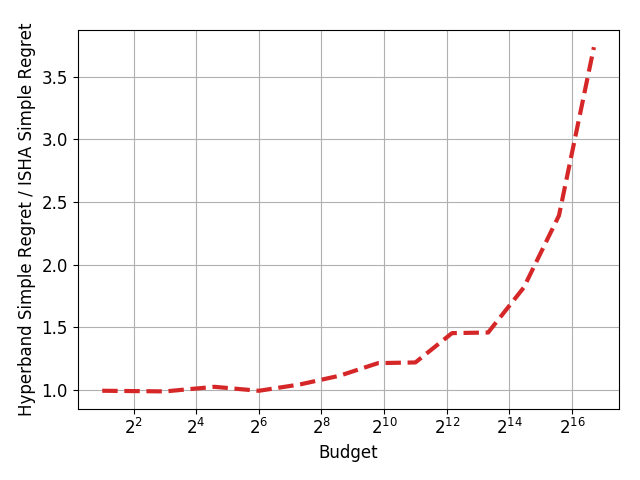
\includegraphics[width=.45\textwidth]{fixedbudget/figures/NY.png}
\caption{The New Yorker dataset. We plot the ratio of state-of-the-art 
Hyperband's simple regret to ISHA's simple regret as a function of
budget. }
\label{fig:isha_vs_hb_improvement}
\vspace{-1.5em}
\end{wrapfigure}

% By allocating budget uniformly in each round of the algorithm to the
% arms with highest empirical means from the last round,
% it naturally avoids spending too much budget on arms which, on the one
% hand, are already performing better than the majority of the population
% and do not yet need further testing,
% or, on the other hand, have performed much worse than the majority of arms and can safely be eliminated.



% Suppose $n$ arms are drawn such that $\mu_i \sim \nu_0$ for $i=1,\dots,n$ and placed in a set $S_0$. 
% At round $k$, each arm $i \in S_k$ is sampled $2^k$ times to obtain an empirical mean $\widehat{\mu}_{i,k}$. 
% The set $S_{k+1}$ is defined to contain the $|S_k|/2 = n 2^{-k}$ arms with the smallest empirical means (breaking ties arbitrarily). 

% Note that at each round $k$ we have $|S_k| = n 2^{-k}$.
% And if 
% \begin{align*}
% n = \arg\max\{ n' \in \mathbb{N} : n' \lceil \log_2 (n') \rceil \leq T \}
% \end{align*}
% then each $t_k = 2^k$. 
% This choice of $n$, given a budget $T$, is the algorithm we will analyze.
% It is remarkable that on the first round, $k=0$, each coin is sampled just a \emph{single} time before half the arms are discarded. 





% Also define
% \begin{align*}
% F_k(x,\mu) = \P\left( \widehat{\mu}_{i,k} \leq x \, | \, \E[\widehat{\mu}_{i,k}] = \mu \right) \quad \text{ and } \quad F_k(x) = \E\left[ \tfrac{1}{|S_k|}\sum_{i \in S_k} \1\{ \widehat{\mu}_{i,j} \leq x) \} \right] = \int F_k(x,\mu) d\nu_k(\mu).
% \end{align*}
% Note that $F_0(x,\mu)$ is the CDF of a single draw of a random variable with mean $\mu$. 
% Likewise, $F_k(x,\mu)$ is equal to $F_0(x,\mu)$ convolved with itself $2^k$ times.

Proving an upper bound for ISHA is challenging because standard
concentration-of-measure approaches do not apply yet in the first
few rounds of the algorithm.
However, based on the proof for Hyperband which requires the budget
from Eq.~\ref{eqn:rough_sample_complexity}
and based on our incomplete theoretical work so far we make the
following conjecture about the simple regret of ISHA.
\begin{conjecture}\label{conjecture:main}
Fix $\delta \in (0,1)$. Under some benign assumptions, for any $\epsilon >0$ define
$z_{n,\epsilon}:= \frac{1}{\epsilon^2} + \frac{1}{\nu_0(\mu_* + \epsilon)}\int_{x = \mu_* + \epsilon}^\infty  \frac{1}{(x-\mu_*)^{2}}  d\nu_0(x)$ (up to logarithmic factors).
%
If Successive Halving of Figure~\ref{alg-SH} is run with $n$ arms and $T=\lceil n \log_2(n) \rceil$ total pulls where $n \geq z_{n,\epsilon}$ then with probability at least $1-\delta$ the single arm returned is no greater than $\mu_* +\epsilon$.
\end{conjecture}

%\subsection{Analysis}
%Our main result relies on two assumptions about the distribution $\phi(\ \cdot \ ; \mu)$ of observations from an arm given a drawn mean $\mu$.
%We make no assumptions about the shape or regularity of the reservoir $\nu_0$.
%% For instance, $\phi(\mu) = \mathcal{N}(\mu,1)$ or $\phi(\mu) = \text{Bernoulli}(\mu)$. 
%\begin{assumption} \label{asm:stochastic_ordering}
%% Let $\phi(\mu)$ denote the probability law that observations from an arm with mean $\mu$ obey. 
%For all $m \in \mathbb{N}$ and $t \in \R$
%\begin{align*}
%\P\Big(\frac{1}{m} \sum_{j=1}^m X_j \leq t \, \Big| \, X_j \overset{iid}{\sim} \phi( \ \cdot \ ; x) \Big) \geq \P\Big(\frac{1}{m} \sum_{j=1}^m Y_j \leq t \, \Big| \, Y_j \overset{iid}{\sim} \phi( \ \cdot \ ; y) \Big) \iff x \leq y.
%\end{align*} 
%\end{assumption}
%Assumption~\ref{asm:stochastic_ordering} states that the distribution with the smaller mean is more likely to have a smaller empirical mean. 
%This holds, for example, if $\phi(\cdot,\mu)$ is $\text{Bernoulli}(\mu)$ or Gaussian observations with known variance $\mathcal{N}(\mu,R)$.
%A consequence of Assumption~\ref{asm:stochastic_ordering} is that
%\begin{align*}
%\P( \mu_i \in S_{k+1} \, | \, \mu_i = x, \mu_i \in S_{k} ) \geq \P( \mu_i \in S_{k+1} \, | \, \mu_i = y, \mu_i \in S_{k} ) \quad \forall x \leq y.
%\end{align*} 
%Assumption~\ref{asm:stochastic_ordering} often holds for the class of single-parameter exponential families that are well-studied in the multi-armed bandit literature \citep{audibert2010best}.
%Our second assumption is standard and allows us to rely on the concentration of measure phenomenon.
%\begin{assumption}\label{asm:subgauss}
%If $X \sim \phi(\ \cdot \ ; \mu)$ then $X-\mu$ is an i.i.d. mean-zero, $R$-sub-Gaussian random variable such that $\E[\exp(\lambda (X-\mu))] \leq \exp(\lambda^2 R /2 )$ for any $\lambda >0$.
%\end{assumption} 
%Assumption~\ref{asm:subgauss} is quite benign: if $X \in [0,1]$ then $R \leq 1/4$; if $X \sim \mathcal{N}(\mu,v^2)$ then $R = v^2$.
%
%\begin{theorem}\label{thm:main}
%Fix $\delta \in (0,1)$. Under Assumptions 1 and 2, for any $\epsilon >0$ define
%\begin{align*}
%z_{n,\epsilon} :=& \frac{\log(2 \log_2(n)/\delta)}{  \nu_0(\mu_* + \epsilon)} \max\left\{ 1, 64 R \log(4 n \log_2(n) /\delta) \sup_{x \geq \mu_* + \epsilon}  (x-\mu_*)^{-2}  \nu_0(x) \right\}\\
%\leq& \log(2 \log_2(n)/\delta) \max\Bigg\{ \frac{1}{\nu_0(\mu_* + \epsilon)},
%\\ &~~~~~~~~~~
%64 R \log(4 n \log_2(n) /\delta) \left( \epsilon^{-2} + \frac{1}{\nu_0(\mu_* + \epsilon)}\int_{x = \mu_* + \epsilon}^\infty  \frac{1}{(x-\mu_*)^{2}}  d\nu_0(x) \right) \Bigg\}.
%\end{align*}
%If Successive Halving of Figure~\ref{alg-SH} is run with $n$ arms and $T=\lceil n \log_2(n) \rceil$ total pulls where $n \geq z_{n,\epsilon}$ then with probability at least $1-\delta$ the single arm returned is no greater than $\mu_* +\epsilon$.
%\end{theorem}
%
%\begin{remark}
%Note that if the support of $\phi$ is bounded in $[0,1]$ then taking $\delta=\epsilon$ in the above theorem implies $\E[ \mu_{J_{T}} ] - \mu_*\leq 2 \epsilon$ whenever $T=\lceil n \log_2(n) \rceil$ and $n \geq z_{n,\epsilon}$.
%\end{remark}
%
%% \begin{theorem}\label{thm:main}
%% Fix $\delta \in (0,1)$ and assume Assumptions 1 and 2 hold.
%% Define 
%% \begin{align*}
%% \Delta_\ell := 2\sqrt{\frac{2R \log(n \log_2(n) 2^{-\ell+2}/\delta)}{2^\ell}} \ , \qquad\qquad \forall \ell \in \{0,1,\dots,\log_2(n)-1\}.
%% \end{align*}
%% If 
%% \begin{align*}
%% n \geq z_n :=& \max_{k=0,1,\dots,\log_2(n)-1} \frac{\log(2 \log_2(n)/\delta)}{  \nu_0(\mu_* + \Delta_k)} \max\{ 1, \max_{\ell=0,\dots,k-1} 2^{\ell+1} \nu_0(\mu_* + 2\Delta_{\ell}) \}
%% \end{align*}
%% then with probability at least $1-\delta$
%% \begin{align*}
%% \mu_{A} \leq  \min_{i \in S_k} \mu_i + \Delta_k/2 \leq \mu_* + \tfrac{3}{2} \Delta_k \quad \text{where} \quad A = \arg\min_{i \in S_k} \widehat{\mu}_{i,k}
%% \end{align*} 
%% for all $k = 0, 1, \dots, \log_2(n)-1$.
%% \end{theorem}
%% We can make the theorem more interpretable by simplifying $z_n$
%% \begin{align*}
%% \max_{\ell=0,\dots,k-1}  2^{\ell+1} \nu_0(\mu_* + 2\Delta_{\ell}) &= \max_{\ell=0,\dots,k-1}  16 R \log(n \log_2(n) 2^{-\ell+2}/\delta) \Delta_{\ell}^{-2}  \nu_0(\mu_* + 2\Delta_{\ell}) \\
%% &\leq  64 R \log(4 n \log_2(n) /\delta) \max_{\ell=0,\dots,k-1}  (2\Delta_{\ell})^{-2}  \nu_0(\mu_* + 2\Delta_{\ell}) \\
%% &\leq  64 R \log(4 n \log_2(n) /\delta) \sup_{x \geq \mu_* + \Delta_{k-1}}  (x-\mu_*)^{-2}  \nu_0(x).
%% \end{align*}
%% We note that
%% \begin{align*}
%% \max_{k=0,1,\dots,\log_2(n)-1} &\frac{\log(2 \log_2(n)/\delta)}{  \nu_0(\mu_* + \Delta_k)} \max\{ 1, \max_{\ell=0,\dots,k-1} 2^{\ell+1} \nu_0(\mu_* + 2\Delta_{\ell}) \}\\
%% \leq& \max_{k=0,1,\dots,\log_2(n)-1} \frac{\log(2 \log_2(n)/\delta)}{  \nu_0(\mu_* + \Delta_k)} \max\left\{ 1, 64 R \log(4 n \log_2(n) /\delta) \sup_{x \geq \mu_* + \Delta_{k-1}}  (x-\mu_*)^{-2}  \nu_0(x) \right\} \\
%% \leq& \frac{\log(2 \log_2(n)/\delta)}{  \nu_0(\mu_* + \Delta_{\log_2(n)-1})} \max\left\{ 1, 64 R \log(4 n \log_2(n) /\delta) \sup_{x \geq \mu_* + \Delta_{\log_2(n)-1}}  (x-\mu_*)^{-2}  \nu_0(x) \right\}
%% \end{align*}
%
%% If we set $\epsilon = \Delta_{\log_2(n)-1}$ and define 
%% \begin{align*}
%% z_{n,\epsilon} :=& \frac{\log(2 \log_2(n)/\delta)}{  \nu_0(\mu_* + \epsilon)} \max\left\{ 1, 64 R \log(4 n \log_2(n) /\delta) \sup_{x \geq \mu_* + \epsilon}  (x-\mu_*)^{-2}  \nu_0(x) \right\}\\
%% \leq& \frac{\log(2 \log_2(n)/\delta)}{  \nu_0(\mu_* + \epsilon)} \max\left\{ 1,  64 R \log(4 n \log_2(n) /\delta) \left( \epsilon^{-2} \nu_0(\mu_*+\epsilon) + \int_{x = \mu_* + \epsilon}^\infty  \frac{1}{(x-\mu_*)^{2}}  d\nu_0(x) \right) \right\} \\
%% =& \log(2 \log_2(n)/\delta) \max\left\{ \frac{1}{\nu_0(\mu_* + \epsilon)}, 64 R \log(4 n \log_2(n) /\delta) \left( \epsilon^{-2} + \frac{1}{\nu_0(\mu_* + \epsilon)}\int_{x = \mu_* + \epsilon}^\infty  \frac{1}{(x-\mu_*)^{2}}  d\nu_0(x) \right) \right\}
%% \end{align*}
%% then the algorithm outputs an $\tfrac{3}{2}\epsilon$-good arm with with probability at least $1-\delta$ whenever $n \geq z_{n,\epsilon}$.
%
%
%Before we prove the theorem, we need some notation and technical lemmas.
%Define 
%\begin{align*}
%\nu_k(x) = \E\Big[ \tfrac{1}{|S_k|} \sum_{i \in S_k} \1\{ \mu_i \leq x \} \Big] = \P( \mu_i \leq x \, | \, \mu_i \in S_k )
%\end{align*}
%where the expectation is taken with respect to the random set $S_k$. 
%Note that this definition is consistent with the reservoir distribution $\nu_0( \, \cdot \, )$ for $k=0$.
%Also define
%\begin{align*}
%\Delta_\ell := 2\sqrt{\frac{2R \log(n \log_2(n) 2^{-\ell+2}/\delta)}{2^\ell}} \ , \qquad\qquad \forall \ell \in \{0,1,\dots,\log_2(n)-1\}.
%\end{align*}
%
%The next lemma follows by a straightforward union and Chernoff bound (Section~\ref{sec:concentration_in_k_proof}).
%\begin{lemma}\label{lem:concentration_in_k}
%Under Assumption~\ref{asm:subgauss} we have
%% \begin{align*}
%$\P\left( \bigcup_{\ell=0}^{\log_2(n)-1} \bigcup_{i \in S_{\ell}} \left\{ |\widehat{\mu}_{i,\ell} - \mu_\ell| \geq \Delta_\ell/2 \right\} \right) \leq \delta/2$.
%% \end{align*}
%\end{lemma}
%
%The next lemma exploits the fact that each $\mu_i \in S_k$ for any $k$ is an i.i.d. draw from $\nu_k$, by definition, and $|S_k| = n 2^{-k}$.
%The result follows by a union bound over $k$ (Section~\ref{sec:good_arms_in_set_k_proof}).
%\begin{lemma}\label{lem:good_arms_in_set_k}
%For any $\ell=0,1,\dots,\log_2(n)-1$ if  $n \geq \xi_{n,\ell} := \frac{\log(2 \log_2(n)/\delta)}{2^{-\ell} \nu_\ell(\mu_* + \Delta_\ell)}$ then 
%% If $n \geq \max_{\ell =0,1,\dots, \log_2(n)-1} \frac{\log(2 \log_2(n)/\delta)}{2^{-\ell} \nu_\ell(\mu_* + \Delta_\ell)}$ then
%\begin{align*}
%\P\Big(\min_{i \in S_\ell} \mu_i > \mu_* + \Delta_\ell \Big) \leq \tfrac{\delta}{2 \log_2(n)}.
%\end{align*}
%Moreover, $\P\Big( \bigcup_{\ell=0}^{\log_2(n)-1} \left\{ \min_{i \in S_\ell} \mu_i > \mu_* + \Delta_\ell \right\} \Big)\leq \frac{\delta}{2}$
%whenever $n \geq \max_{\ell=0,1,\dots,\log_2(n)-1} \xi_{n,\ell}$.
%\end{lemma}
%
%
%If $n \geq  \max_{\ell=0,1,\dots,\log_2(n)-1} \frac{\log(2 \log_2(n)/\delta)}{2^{-\ell} \nu_\ell(\mu_* + \Delta_\ell)}$, then combining the two above lemmas would give the desired result of Theorem~\ref{thm:main}.
%However, $\nu_k$ is not a natural quantity to reason about since it depends on the behavior of the algorithm.
%The next two lemmas characterize the behavior of this evolving distribution.
%The proof of the following lemma applies Bayes rule and exploits Assumption~\ref{asm:stochastic_ordering}. 
%It comes to the intuitive conclusion that the distribution of the true means gets no worse by thresholding the empirical means at the median (Section~\ref{sec:core_lemma_proof}).
%\begin{lemma}\label{lem:core_lemma}
%Assume Assumption~\ref{asm:stochastic_ordering} holds.
%For any $k$ and $x\in \R$ we have
%\begin{align*}
%\nu_{k+1}(x) &= 2 \P( \mu_i \in S_{k+1} \, | \, \mu_i \leq x, \mu_i \in S_{k} ) \, \nu_k(x)
%\geq \nu_k(x).
%\end{align*}
%Moreover, for any $k$ and $x < y$ we have $\frac{\nu_{k+1}(x)}{\nu_k(x)} \geq \frac{\nu_{k+1}(y)}{\nu_k(y)}$.
%% \begin{align*}
%% \frac{\nu_{k+1}(x)}{\nu_k(x)} \geq \frac{\nu_{k+1}(y)}{\nu_k(y)}.
%% \end{align*}
%\end{lemma} 
%
%\noindent The next lemma refines the previous one, stating sufficient conditions for  improvement. 
%\begin{lemma}\label{lem:E_k}
%Assume Assumption~\ref{asm:stochastic_ordering} holds.
%Fix some $k \in \mathbb{N}$. 
%% Without loss of generality, at stage $k$ we have $\mu_i \sim \nu_k$ for $i \in S_k = \{1,\dots,|S_k|\}$. 
%% The realized random variables $\widehat{\mu}_{i,k}$ are the result of averaging $2^k$ realizations from the base distribution with mean $\mu_i$.  
%Define the event
%\begin{align*}
%\mathcal{E}_k = \{ \min_{i\in S_k} \mu_i-\mu_* \leq \Delta_k, \, \max_{i\in S_k} |\widehat{\mu}_{i,k} - \mu_i| \leq \Delta_k/2\}.
%\end{align*} 
%Then
%\begin{align} 
%\nu_{k+1}(\mu_*+\epsilon) &\geq \1_{\mathcal{E}_k}\min\{ 1, 2 \nu_k(\mu_*+\epsilon) , \tfrac{\nu_0(\mu_*+\epsilon) }{\nu_0(\mu_* + 2\Delta_k)} \} \quad \forall \epsilon \leq \Delta_k. \label{eqn:recursion}
%\end{align}
%\end{lemma}
%\begin{proof}
%Assume $\mathcal{E}_k$.
%We consider two exhaustive cases: 
%
%\noindent\textbf{Case 1}: $\max_{i \in S_{k+1}} \widehat{\mu}_{i,k} \leq \mu_* + \Delta_k + (\Delta_k/2)$. Here 
%\begin{align*}
%\max_{i \in S_{k+1}} \mu_i \leq \max_{i \in S_{k+1}} \widehat{\mu}_{i,k} + \Delta_k/2 \leq \mu_* + 2 \Delta_k
%\end{align*} 
%which means that no $2\Delta_k$-bad arms make it into $S_{k+1}$ and $\nu_{k+1}(\mu_*+2\Delta_k)=1$. Thus, applying the second result of Lemma~\ref{lem:core_lemma} twice with $x = \mu_* + \epsilon$ and $y=\mu_* + 2 \Delta_k$, we have $\nu_{k+1}(\mu_* + \epsilon) \geq \frac{\nu_k(\mu_*+\epsilon)}{\nu_k(\mu_* + 2\Delta_k)} \geq \frac{\nu_0(\mu_*+\epsilon)}{\nu_0(\mu_* + 2\Delta_k)}$ for all $\epsilon < \Delta_k$.
%
%\noindent\textbf{Case 2}: $\mu_* + \Delta_k + (\Delta_k/2) < \max_{i \in S_{k+1}} \widehat{\mu}_{i,k}$ In this case all $\Delta_k$-good arms in $S_k$ are guaranteed to be in $S_{k+1}$. Thus $\nu_{k+1}(\mu_*+\Delta_k) = \min\{1,2 \nu_{k}(\mu_* + \Delta_k)\}$ by the first result of Lemma~\ref{lem:core_lemma} with $x = \mu_* +\Delta_k$.
%% \begin{align*}
%% \mathcal{E}_k \implies \nu_{k+1}(\mu_*+\epsilon) &\geq \min\{ 1, 2 \nu_k(\mu_*+\epsilon) , \tfrac{\nu_k(\mu_*+\epsilon) }{\nu_k(\mu_* + 2\Delta_k)} \} \quad \forall \epsilon \leq \Delta_k.
%% \end{align*}
%\end{proof}
%
%We are now ready to prove Theorem~\ref{thm:main}.
%\begin{proof}
%Let $z_{n,\Delta_{k}}$ be $z_{n,\epsilon}$ from the theorem statement with $\epsilon=\Delta_k$. Define
%% \begin{align*}
%% z_{n,\Delta_{k}}&:= \frac{\log(2 \log_2(n)/\delta)}{  \nu_0(\mu_* + \Delta_{k})} \max\left\{ 1, 64 R \log(4 n \log_2(n) /\delta) \sup_{x \geq \mu_* + \Delta_{k}}  (x-\mu_*)^{-2}  \nu_0(x) \right\}
%% \end{align*}
%% as well as
%\begin{align*}
%z_n := \max_{k=0,1,\dots,\log_2(n)-1} z_{n,\Delta_{k}}= z_{n,\Delta_{\log_2(n)-1}}  \quad \text{and} \quad
%\xi_{n,k} := \frac{\log(2 \log_2(n)/\delta)}{2^{-k} \nu_k(\mu_* + \Delta_k)}
%\end{align*}
%where $\xi_{n,k}$ comes from Lemma~\ref{lem:good_arms_in_set_k}.
%Note that $n \geq z_n$ by assumption.
%The theorem claims that with probability at least $1-\delta$ the returned arm has a mean no greater than $\mu_* + \Delta_{\log_2(n)-1}$ (which is implied if $\mathcal{E}_{\log_2(n)-1}$ holds) whenever $n \geq z_n = z_{n,\Delta_{\log_2(n)-1}}$ by simply making the substitution $\epsilon := \Delta_{\log_2(n)-1}$.
%Thus, our goal is to show that $\mathcal{E}_{\log_2(n)-1}$ holds by proving the stronger statement that $\bigcap_{k=0}^{\log_2(n)-1} \mathcal{E}_k$ holds.
%
%By immediate application of Lemma~\ref{lem:concentration_in_k} and Lemma~\ref{lem:good_arms_in_set_k}, for all $k=0,1,\dots,\log_2(n)-1$ simultaneously
%\begin{align}\label{eqn:main_implication}
%\{n \geq \xi_{n,k}\}  \implies \{ \min_{i \in S_k} \mu_i \leq \mu_* + \Delta_k \} \cap  \{ \max_{i\in S_k} |\widehat{\mu}_{i,k} - \mu_i| \leq \Delta_k/2 \} = \mc{E}_k
%\end{align}
%with probability at least $1-\delta$.
%% Thus, since $n \geq z_n$ it suffices to show that $\bigcap_{k=0}^{\log_2(n)-1} \{z_{n,\Delta_k} \geq \xi_{n,k}\}$.
%In what follows, assume the implication of \eqref{eqn:main_implication} holds for all $k$, since these occur with probability at least $1-\delta$.
%
%We will prove the theorem by induction
%% \begin{align*}
%% \{ n \geq z_n \} \cap \left\{ \bigcap_{\ell=0}^{k-1} \mathcal{E}_\ell \right\} \implies \{ n \geq z_n \} \cap \left\{ \bigcap_{\ell=0}^{k} \mathcal{E}_\ell \right\}
%% \end{align*}
%starting with the base case
%\begin{align*}
%\{n \geq z_n\} \implies \{ n \geq z_{n,\Delta_0} \} \implies \{ n \geq \frac{\log(2 \log_2(n)/\delta)}{ \nu_0(\mu_* + \Delta_0)} \} \equiv \{n \geq \xi_{n,0}\} \overset{\eqref{eqn:main_implication}}{\implies} \mc{E}_0.
%\end{align*} 
%Fix any $k \in \{1,\dots,\log_2(n)-1\}$. 
%Note $\{\nu_k(\mu_*+\Delta_k)=1 \} \implies \left\{ \min_{i \in S_k} \mu_i-\mu_* \leq \Delta_k \right\}$ so
%\begin{align*}
%\{\nu_k(\mu_*+\Delta_k)=1 \} \cap \{ \max_{i\in S_k} |\widehat{\mu}_{i,k} - \mu_i| \leq \Delta_k/2 \} \implies \mathcal{E}_k.
%\end{align*} 
%So assume $\nu_k(\mu_*+\Delta_k)<1$.
%On $\left\{ \bigcap_{\ell=0}^{k-1} \mathcal{E}_\ell \right\}$ we have 
%\begin{align*}
%\nu_{k}(\mu_*+\Delta_k) &\geq \min\{ 1, 2 \nu_{k-1}(\mu_*+\Delta_k) , \tfrac{\nu_0(\mu_*+\Delta_k) }{\nu_0(\mu_* + 2\Delta_{k-1})} \} \\
%&\geq \min\{ 1, 2 \min\{ 1, 2 \nu_{k-2}(\mu_*+\Delta_k) , \tfrac{\nu_0(\mu_*+\Delta_k) }{\nu_0(\mu_* + 2\Delta_{k-2})} \} , \tfrac{\nu_0(\mu_*+\Delta_k) }{\nu_0(\mu_* + 2\Delta_{k-1})} \} \\
%% &= \min\{ 1, 2^2 \nu_{k-2}(\mu_*+\Delta_k) , 2 \tfrac{\nu_0(\mu_*+\Delta_k) }{\nu_0(\mu_* + 2\Delta_{k-2})} , \tfrac{\nu_0(\mu_*+\Delta_k) }{\nu_0(\mu_* + 2\Delta_{k-1})} \} \\
%&\geq \min\{ 1,2^{k} \nu_0(\mu_* + \Delta_k), \min_{\ell=0,\dots,k-1} 2^{k-1-\ell} \tfrac{\nu_0(\mu_*+\Delta_k)}{\nu_0(\mu_* + 2\Delta_{\ell})} \} \\
%&= \min\{ 1,2^{k} \nu_0(\mu_* + \Delta_k) \min\{ 1,   \tfrac{1}{\max_{\ell=0,\dots,k-1} 2^{\ell+1} \nu_0(\mu_* + 2\Delta_{\ell})} \} \}\\
%% &= 2^{k} \nu_0(\mu_* + \Delta_k) \min\{ 1,   \tfrac{1}{\max_{\ell=0,\dots,k-1} 2^{\ell+1} \nu_0(\mu_* + 2\Delta_{\ell})} \} \\
%&= 2^{k} \nu_0(\mu_* + \Delta_k) \tfrac{1}{\max\{ 1, \max_{\ell=0,\dots,k-1} 2^{\ell+1} \nu_0(\mu_* + 2\Delta_{\ell}) \}} 
%\end{align*}
%where the last line uses $\nu_k(\mu_*+\Delta_k)<1$ and moves the $\min$ to the denominator.
%Now
%% \begin{align*}
%% \max\{1, \max_{\ell=0,\dots,k-1}  2^{\ell+1} \nu_0(\mu_* + 2\Delta_{\ell}) \} &= \max\{1, \max_{\ell=0,\dots,k-1}  16 R \log(n \log_2(n) 2^{-\ell+2}/\delta) \Delta_{\ell}^{-2}  \nu_0(\mu_* + 2\Delta_{\ell}) \} \\
%% &\leq \max\{1, 64 R \log(4 n \log_2(n) /\delta) \max_{\ell=0,\dots,k-1}  (2\Delta_{\ell})^{-2}  \nu_0(\mu_* + 2\Delta_{\ell}) \} \\
%% &\leq \max\{1, 64 R \log(4 n \log_2(n) /\delta) \sup_{x \geq \mu_* + \Delta_{k-1}}  (x-\mu_*)^{-2}  \nu_0(x) \} \\
%% &\leq \max\{1, 64 R \log(4 n \log_2(n) /\delta) \sup_{x \geq \mu_* + \Delta_{k}}  (x-\mu_*)^{-2}  \nu_0(x) \} \\
%% &= \frac{\nu_0(\mu_* + \Delta_{k})}{\log(2 \log_2(n)/\delta)} z_{n,\Delta_{k}}.
%% % &\leq \frac{\nu_0(\mu_* + \Delta_{k})}{\log(2 \log_2(n)/\delta)} n .
%% \end{align*}
%\begin{align*}
%\max_{\ell=0,\dots,k-1}  2^{\ell+1} \nu_0(\mu_* + 2\Delta_{\ell}) &= \max_{\ell=0,\dots,k-1}  16 R \log(n \log_2(n) 2^{-\ell+2}/\delta) \Delta_{\ell}^{-2}  \nu_0(\mu_* + 2\Delta_{\ell}) \\
%&\leq 64 R \log(4 n \log_2(n) /\delta) \max_{\ell=0,\dots,k-1}  (2\Delta_{\ell})^{-2}  \nu_0(\mu_* + 2\Delta_{\ell}) \\
%&\leq 64 R \log(4 n \log_2(n) /\delta) \sup_{x \geq \mu_* + \Delta_{k-1}}  (x-\mu_*)^{-2}  \nu_0(x) \\
%&\leq 64 R \log(4 n \log_2(n) /\delta) \sup_{x \geq \mu_* + \Delta_{k}}  (x-\mu_*)^{-2}  \nu_0(x),
%\end{align*}
%% so that
%\begin{align*}
%\max\{1, \max_{\ell=0,\dots,k-1}  2^{\ell+1} \nu_0(\mu_* + 2\Delta_{\ell}) \}
%&\leq \max\{1, 64 R \log(4 n \log_2(n) /\delta) \sup_{x \geq \mu_* + \Delta_{k}}  (x-\mu_*)^{-2}  \nu_0(x)\} \\
%&=\tfrac{\nu_0(\mu_* + \Delta_{k})}{\log(2 \log_2(n)/\delta)} z_{n,\Delta_{k}}.
%% &\leq \frac{\nu_0(\mu_* + \Delta_{k})}{\log(2 \log_2(n)/\delta)} n .
%\end{align*}
%Plugging this result back into the previous display and rearranging, we obtain
%\begin{align*}
%\nu_{k}(\mu_*+\Delta_k) \geq \frac{2^k \log(2 \log_2(n)/\delta)}{z_{n,\Delta_{k}}} \equiv z_{n,\Delta_k} \geq \xi_{n,k}.
%\end{align*}
%Thus,
%\begin{align*}
%\{n \geq z_n \} \cap \left\{ \bigcap_{\ell=0}^{k-1} \mathcal{E}_\ell \right\} &\implies \{n \geq z_n \} \cap \{z_{n,\Delta_k} \geq \xi_{n,k} \} \cap \left\{ \bigcap_{\ell=0}^{k-1} \mathcal{E}_\ell \right\}  \overset{\eqref{eqn:main_implication}}{\implies} \{n \geq z_n \} \cap  \left\{ \bigcap_{\ell=0}^{k} \mathcal{E}_\ell \right\}
%\end{align*}
%Because $k$ was chosen arbitrarily, and because $\mc{E}_0$ holds, we have proven that 
%$\{n \geq z_n \} \implies \left\{ \bigcap_{\ell=0}^{\log_2(n)-1} \mathcal{E}_\ell \right\}$ 
%with probability at least $1-\delta$.
%\end{proof}


\subsection{Lower Bound}

We will now prove a lower bound for the problem which ISHA solves.
Fix any reservoir distribution $\nu_0$ and $\epsilon,\delta \in (0,1)$. 
Our proposed upper bound of Conjecture~\ref{conjecture:main} states that if ISHA is provided a budget of $\epsilon^{-2} + \frac{1}{\nu_0(\mu_* + \epsilon)}\int_{\mu_*+\epsilon} (\mu-\mu_*)^{-2} d\nu_0(\mu)$ pulls (up to logarithmic factors), then the prescribed procedure outputs an $\epsilon$-good arm with probability at least $1-\delta$.
In this section, we argue that any algorithm that identifies an $\epsilon$-good arm with probability at least $1-\delta$ must take nearly this many total pulls in expectation.
We follow the lower bound technique of \cite{malloy2012quickest} beginning with a definition borrowed from \cite{berry1997}.
\begin{definition}
% Fix any $\nu_0$ and $\epsilon,\delta\in(0,1)$.
A \emph{non-recalling strategy} is one that always draws a new arm from $\nu_0$ when switching from the current arm and never pulls a previous arm again.
% At each time the procedure recommends the arm being currently pulled.  
\end{definition}

Implicit in \cite{malloy2012quickest} is the assumption that there exists a non-recalling strategy for every $\nu_0, \epsilon, \delta$ that is near-optimal with respect to \emph{any} strategy.
Such an assumption is reasonable because observations from any particular arm are conditionally independent given the mean of the arm, and knowing the mean of one arm provides no information about the mean of another. 
Thus, the number of times any particular arm is pulled depends \emph{only} on the observations from that arm, and because the means of the arms are drawn i.i.d. from $\nu_0$, each arm should be treated identically.
Thus, the procedure will continue to discard arms until it finds one and commits to it for all time. 
Of course, any such non-recalling strategy would require precise knoweldge of $\nu_0$ making it purely a thought experiment, but it is useful for a lower bound.
Nevertheless, many algorithms for the regret setting of infinite-armed bandits make very strong assumptions and are non-recalling strategies (c.f., \cite{berry1997,bonald2013two,Chan2018Infinite}.

% The only reason for exploration in bandits is to discover what \emph{else} is out there, but in this case the player knows $\nu$ exactly, so they already \emph{know} what else is out there. 
% Thus, we only need to consider algorithms that act on one arm at a time, and treat each arm identically. 
Define
$KL(\mu,\mu') = \int_{x} \phi(x;\mu) \log\left( \frac{\phi(x;\mu)}{\phi(x;\mu')}\right) dx$
where we assume $KL(c,d) \geq KL(a,b)$ for all $[a,b] \subseteq [c,d]$.
This is a common assumption and holds for families of distributions $\phi( \cdot ; \mu)$ parameterized by their mean (e.g., Bernoulli, Gaussian, Poisson; \cite{kaufmann2016complexity}).
\begin{theorem}\label{thm:fb-lb}
Fix a reservoir distribution $\nu$, $\delta \in (0,1/15)$, and $\epsilon >0$ such that $\nu(\mu_*+\epsilon) \leq 1/2$.
If at time $\tau \in \mathbb{N}$ a non-recalling strategy outputs an arm $\widehat{i} \in \mathbb{N}$ that satisfies $\P(\mu_{\widehat{i}} \leq \mu_* + \epsilon ) \geq 1-\delta$, then
\begin{align*}
\E[ \tau ] &\geq (1-\delta)\frac{  \log(\tfrac{(1-\delta)\widetilde{\kappa}}{e \delta \nu(\mu_*+\epsilon)})}{KL(\mu_* , \widetilde{\mu})}  - \frac{2}{KL(\mu_* + \epsilon, \mu_*)}  + \frac{3/8}{\nu(\mu_*+\epsilon)} \int_{\mu_*+\epsilon} \frac{1}{KL(\mu,\mu_*)} d\nu(\mu) 
\end{align*}
for any $\widetilde{\mu}$ with $\widetilde{\kappa} := \nu(\widetilde{\mu}) - \nu(\mu_*+\epsilon) > \frac{ \delta \nu(\mu_*+\epsilon)}{1-\delta}$
\end{theorem}


\noindent We related this lower bound to previously known upper bounds using Gaussian realizations (or Bernoullis near $1/2$) where $KL(\mu,\mu') \leq c (\mu-\mu')^2$: 

\noindent\textbf{Continuous as $\mu \rightarrow \mu_*$:} Take $\widetilde{\kappa} = \sqrt{\delta}$. As $\delta \rightarrow 0$ we have $\widetilde{\mu} \rightarrow \mu_*+\epsilon$ to yield a sample compelxity of $\epsilon^{-2} \log(\tfrac{1}{ \delta \nu(\mu_*+\epsilon)}) + \frac{1}{\nu(\mu_*+\epsilon)} \int_{\mu_*+\epsilon} \frac{1}{(\mu-\mu_*)^2} d\nu(\mu)$.

\noindent\textbf{Two spike, Equation~\ref{eqn:mostbiasedcoin_reservoir}:} Take $\widetilde{\kappa} = (1-\pi)$ to yield a sample complexity of $\epsilon^{-2} \log(\tfrac{1}{\pi \delta}) + \frac{1}{\pi \epsilon^2}$.

\noindent\textbf{Polynomial-tail, Equation~\ref{eqn:beta_parameterization}:} $\nu(\mu_* + x) := \P( \mu \leq \mu_* + x) \propto x^\beta$. Take $\widetilde{\mu} = \mu_* + 2^{1/\beta} \epsilon$ so that $\widetilde{\kappa} = \nu(\mu_*+2^{1/\beta} \epsilon) - \nu(\mu_* + \epsilon) \propto \epsilon^\beta$ yielding a sample complexity of $\epsilon^{-2}\log(1/\delta) + \epsilon^{-\beta}$.

We will only sketch the proof of Theorem~\ref{thm:fb-lb}, leaving the technical details to Section~\ref{sec:SHproof}.
Since each arm is treated identically, one realizes that such a procedure is performing a sequence of composite binary hypothesis tests where the test decides to keep sampling or not given the observations up to the current time.
Let $\P_\mu$ and $\E_\mu$ be the probability law of observations from an arm with mean $\mu$.
It will be also convenient to define $\pi:=\nu(\mu_*+\epsilon)$.
Let $N_i$ be the random number of times the $i$th arm is pulled before it is either discarded (denoted by the event $R_i^c$) or declared as $\epsilon$-good ($R_i$). 
Note that $R_i$, $R_1$ as well as $N_i$, $N_1$ for all $i$ are independent and identically distributed for any non-recalling algorithm by the i.i.d. nature of the draws from $\nu_0$.
Define $\alpha := \frac{1}{1-\pi} \int_{\mu_1 = \mu_* + \epsilon} \P_{\mu_1}(R_1) d\nu(\mu_1)$ and $\beta := \frac{1}{\pi} \int_{\mu_1 = \mu_*}^{\mu_* + \epsilon} \P_{\mu_1}(R_1^c) d\nu(\mu_1)$.
Then
\begin{align*}
\E[\tau] = \E[ \sum_{i \geq 1} N_i ]
 &= \E[N_1] + \E[\sum_{i > 1} N_i | R_1^c] ( (1-\alpha) (1-\pi) + \beta \pi) \\
&= \E[N_1] + \E[\sum_{i \geq 1} N_i ] ( (1-\alpha) (1-\pi) + \beta \pi) 
\end{align*}
by the i.i.d. nature of $\mu_i \sim \nu$ and thus memoryless property of the process.
After rearranging,
\begin{align}
\E[ \sum_{i \geq 1} N_i ] &= \frac{\E[N_1]}{\alpha (1-\pi) + (1-\beta) \pi}. \label{eqn:N1_to_many}
\end{align}

\begin{lemma}\label{lem:exp_N1}
Fix $\alpha,\beta \in (0,1)$. 
For any $\kappa \in (\frac{\alpha(1-\pi)}{1-\beta},1)$
\begin{align*}
\E[ N_1 ] \geq&  \frac{\pi  d(1-\beta,  \tfrac{\alpha(1-\pi)}{\widetilde{\kappa}})}{KL(\mu_*,\widetilde{\mu})} + d(\tfrac{\alpha(1-\pi)}{\kappa} , 1-\beta ) \left(  \frac{-\kappa}{KL(\mu_* + \epsilon, \mu_*)}  + \frac{1}{2} \int_{\mu_*+\epsilon} \frac{1}{KL(\mu,\mu_*)} d\nu(\mu) \right) 
\end{align*}
for any $\widetilde{\mu}$ satisfying $\widetilde{\kappa}:=\nu(\widetilde{\mu}) - \nu(\mu_*+\epsilon) > \frac{\alpha(1-\pi)}{1-\beta}$.
\end{lemma}
A similar calculation to \eqref{eqn:N1_to_many} reveals
% \begin{align*}
$\P(\mathrm{error}) = \P( \bigcup_{i\geq 1} \{ R_i, \mu_i > \mu_* + \epsilon \} ) = \frac{ \alpha(1-\pi)}{(1-\beta)\pi + \alpha(1-\pi)}$ 
% \end{align*}
and rearranging we observe that for some $\delta \in (0,1)$
\begin{align} \label{eqn:error_implication}
\P(\mathrm{error}) 
= \frac{1}{1 + \frac{\pi(1-\beta)}{(1-\pi)\alpha}} \leq \delta \iff \frac{(1-\pi)\alpha}{\pi(1-\beta)} \leq \frac{\delta}{1-\delta}.
\end{align}
If $\kappa = 2 \pi$ and $\P(\mathrm{error})\leq \delta$ then by the above implication, 
% \begin{align*}
$\kappa = 2\pi > 2 \tfrac{\pi \delta}{1-\delta} \overset{\eqref{eqn:error_implication}}{\geq} 2 \tfrac{(1-\pi)\alpha}{1-\beta} > \tfrac{(1-\pi)\alpha}{1-\beta}$
% \end{align*}
where the last strict inequality is precisely the condition on $\kappa$ for which Lemma~\ref{lem:exp_N1} applies.
Thus, we plug in the result of Lemma~\ref{lem:exp_N1} with $\kappa=2\pi$ into Equation~\ref{eqn:N1_to_many} and simplify to obtain the theorem.






